\documentclass{kecsmstr}
\usepackage{graphicx, epstopdf, amsmath, amssymb, color, caption, subcaption, comment, booktabs, mathabx, mathtools, varwidth}
\usepackage[algo2e, noend, noline, linesnumbered]{algorithm2e}
\DeclarePairedDelimiter{\ceil}{\lceil}{\rceil}
\DeclarePairedDelimiter{\floor}{\lfloor}{\rfloor}
\DeclareMathOperator*{\argmin}{arg\,min}
\DontPrintSemicolon
\newcommand{\bE}{\mathbb{E}}
\newcommand{\bI}{\mathbb{I}}
\newcommand{\cA}{\mathcal{A}}
\newcommand{\cC}{\mathcal{C}}
\newcommand{\cD}{\mathcal{D}}
\newcommand{\cI}{\mathcal{I}}
\newcommand{\cN}{\mathcal{N}}
\newcommand{\cO}{\mathcal{O}}
\newcommand{\cS}{\mathcal{S}}
\newcommand{\cT}{\mathcal{T}}
\newcommand{\cZ}{\mathcal{Z}}
\newcommand{\eg}{{\it e.g.,}~}
\newcommand{\ie}{{\it i.e.,}~}
\newcommand{\mctssr}{MCTS_{\mathcal{S}\mathcal{R}}}

\newcommand{\redbold}[1]{\textbf{\color{red}#1}}

\newcommand{\toexpand}[1]{{\it $\ll$ #1 ... $\gg$ }} 

\newcommand\NoIndent[1]{%
  \par\vbox{\parbox[t]{\linewidth}{#1}}%
}

\graphicspath{{img/}}
\DeclareGraphicsExtensions{.pdf,.jpg,.png,.eps}

\newcommand{\keywords}[1]{\par\addvspace\baselineskip
\noindent\keywordname\enspace\ignorespaces#1}

\title{Novel Selection Methods For Monte-Carlo Tree Search}
\author{Tom Pepels}

\thesistype{Master of Science of Artificial Intelligence}

\thesisdate{June 2014} \thesisnumber{14-00}

%Thesiscommittee: use \\ to separate members
\committee{Dr.~Mark~H.M. Winands\\
           Dr.~Marc~Lanctot}
% ================================

\begin{document}

% leave this in place! =============
\makeheaders \pagenumbering{roman} \maketitle \setcounter{page}{2}
\emptypage
% ================

\chapterx{Preface} 
In this thesis I present the result of my investigation into simple regret minimization for Monte-Carlo Tree Search. The thesis present the motivation, background and formal definition of a novel search algorithm based on minimizing both simple and cumulative regret. The algorithm was developed for, and tested in four two-player games: Amazons, Breakthrough, Chinese Checkers and Pentalath. The research was performed at the Department of Knowledge Engineering, Maastricht University, The Netherlands.

Special thanks goes to both Dr. Mark Winands and Dr. Marc Lanctot for providing the inspiration and guidance required to develop this novel algorithm. Their combined, vast experience was crucial to obtain the results presented in this work. Moreover, I would like to thank my wife Priscilla for her support, and for  bearing with me during the research. Without both her emotional and financial assistance you would not be reading this thesis.
\newline \newline

\noindent Tom Pepels \newline
Maastricht, May 2014
\emptypage

\chapterx{Summary} \emptypage

\tableofcontents  \emptypage \pagenumbering{arabic}

\chapter{Introduction}

\begin{chaptercontents} An overview of Monte-Carlo Tree Search and the main topic of this thesis, simple regret minimization applied to Monte-Carlo Tree Search. Moreover, the problem statement and research questions are drafted and a general outline of the structure of the thesis is given.
\end{chaptercontents}

\section{Artificial Intelligence and Games}
Decision making and problem solving have been a core topic in Artificial Intelligence (AI) since its birth over half a century ago. In many domains an agent is required to find a specific sequence of actions to achieve a certain goal. When such a problem is defined as a graph or a tree, a search algorithm can be used to explore the state-space to find rewarding states in the future and find the best action given the current state.
Given that most real domains are too complicated to result in a limited, specific set of rules for the agent to follow, an abstract domain is more appropriate when investigating search algorithms. For a single agent, puzzles, graph-problems and simplified real-world models are often investigated. In this case, the agent's goals are non-adversarial, it maximizes utility over time to reach a set goal. When more than one agent is involved, games provide adversarial challenges with simple rules that result in large and complex state-spaces. For most interesting games, an exhaustive search is not feasable but well-playing algorithms have been found.

Even before the first computer capable of playing games at a reasonable level was developed, Alan Turing was thinking about computer chess~\citebay{turing1988chess}. Over the decades, faster computers allowed for deeper investigation into game-playing algorithms such as $\alpha\beta$~\citebay{knuth1976analysis}, Principal-Variation Search~\citebay{marsland1983relative}, Proof-number search~\citebay{allis1994proof}. One of the reasons game AI research has sparked interest over the years is that algorithms can be directly measured against human players. In 1997 {\sc Deep Blue}~\citebay{campbell2002deep} defeated then-reigning World Chess Champion Garry Kasparov in a six-game match, the first time an algorithm beat a human champion. After plentiful research had been performed in computer Chess, Go was the next target for game AI research. In contrary to Chess, for Go it is not straightforeward to find even a simple evaluation function. Moreover, Go's branching factor is not limited by its rules, over the course of the game stones can be played anywhere on the board leading to a high branching factor.

With the introduction of Monte-Carlo Tree Search~\citebay{kocsis2006bandit,coulom2007efficient}, and UCT~\citebay{kocsis2006bandit}, reasearchers could reach human level play in Go~\citebay{lee2010current} on small boards. Since it requires no static heuristic evaluation, using simulations to determine the rewards of states in the tree, and a selection policy to explore the tree, MCTS performed better than any algorithm had before. The success of MCTS and UCT in Go sparked researchers' interests in developing a better understanding of the algorithm and applying it to different domains ranging from games, planning problems and real-time domains~\citebay{browne2012survey}.

\section{Monte-Carlo Tree Search}
Monte-Carlo Tree Search (MCTS) is a best-first search method based on random sampling by Monte-Carlo simulations of the state space for a specified domain~\citebay{coulom2007efficient,kocsis2006bandit}. In gameplay, this means that decisions are made based on the results of randomly simulated play-outs. MCTS has been successfully applied to various turn-based games such as Go~\citebay{lee2010current}, Lines of Action~\citebay{Winands2010b}, and Hex~\citebay{arneson2010monte}. Moreover, MCTS has been used for agents playing real-time games such as the Physical Traveling Salesman~\citebay{powleytsp}, real-time strategy games~\citebay{balla2009uct}, and Ms~Pac-Man~\citebay{realtime2014}, but also in real-life domains such as optimization, scheduling, and security~\citebay{browne2012survey}.

MCTS builds a tree online by iteratively sampling the state space of the domain. At each iteration, a selection policy chooses a path in the tree. When a leaf is reached, it is expanded to reveal the next possible states. A simulated play-out is then initiated at one of the new leafs. The result of this playout, \eg a win, loss or draw, is backpropagated to the root of the tree. Finally, after a set computational limit is reached, \eg a time, memory or simulation limit, the statistics gathered at the first ply determine which move to play.

\section{Regret Minimization}
The driving force behind MCTS is the notion of regret minimization. Algorithms used in multi-armed bandit (MAB) research have been developed to minimize cumulative regret. UCB~\citebay{auer2002using} is a selection policy for the MAB problem, which minimizes cumulative at a fast rate, converging to the empirically best arm fast. Once the best arm is found by exploring the available options, it exploits it by repeatedly pulling that arm, minimizing overall cumulative regret. This policy was adapted to be used in MCTS in the form of UCT~\citebay{kocsis2006bandit}

Recently, simple regret has been proposed as a new criterion for assessing the performance of both MAB~\citebay{audibert2010best,Bubeck11Pure} and MCTS~\citebay{tolpin2012mcts,Feldman12BRUE} algorithms. This is a naturally fitting quantity to opitmize in the MCTS setting. All simulations executed by MCTS are for the purpose of learning good moves. However, the final move chosen after all simulations are performed, \ie the \emph{recommendation}, is the one that has real consequences. Therefore, the choice of this move should have an as low as possible simple regret. Moreover, once MCTS finds a good move with high certainty, the utility of re-selecting that move diminishes over time. When a promising node, or group of nodes is visited too often, at a certain point insufficient simulation time remains to determine whether there exists a viable alternative. Rather it may be favorable to explore other options more, even if a single move is identified as the best. At the same time, MCTS should not `waste' its time one moves that are known to be bad.

This is the driving idea behind full exploration algorithms such as Successive Rejects~\citebay{audibert2010best} and Sequential Halving~\citebay{Karnin13SH}. Contrary to UCB, these algorithms have no specific exploitation phase, they divide their time uniformly between a continuously reduced set of options. The final recommendation is the single arm that remains after all trials are finished.

\section{Problem Statement and Research Questions}
On the one hand, simple regret optimization (full exploration) has practical problems in games, especially at low search times. On the other hand, algorithms based on cumulative regret perform particularly well in comparison under these limited circumstances. Based on the assumption that simple regret is a better way to determine a move's utility, and that full exploration algorithms can be used recursively, we may be able to develop an algorithm that utilizes both types of regret to improve the performance of MCTS. Given that current algorithms are either designed to minimize one type of regret, or fall short in improving performance in games. The problem statement of this thesis is:
\newline \newline
\emph{How can a Monte-Carlo Tree Search algorithm be constructed that minimizes both simple and cumulative regret in their appropriate contexts?}
\newline \newline
The following four research questions arise from this problem statement:
\begin{enumerate}

\item{\emph{How can a search algorithm be developed for minimizing both simple and cumulative regret in a game tree?}}
\item{\emph{At which point should we switch from simple to cumulative regret minimization in the tree?}}
\newline
\NoIndent{To answer these questions, an investigation into curent state-of-the-art multi-armed bandit algorithms is required. Additionaly, some MCTS algorithms already minimize simple regret, but have not shown general improvement in games. However, these algorithms may still prove a usefull baseline.
Next, our initial assumption regarding simple regret minization in games ought to be verified:}

\item{\emph{Will using simple regret minimizing, full exploration algorithms in MCTS improve performance in two player games?}}
\newline
\NoIndent{This question will be answered by experimentation in four different two player games: Amazons, Breakthrough, Chinese Checkers and Pentalath.

Which leads to the question whether the current foundation of MCTS research is still appropriate in the context of simple regret minimization:}
\item{\emph{Can well-known MCTS enhancements such as MCTS-Solver, Progressive History and MAST be used (more) effectively in the new algorithm?}}
\end{enumerate}

\noindent This question is crucial for the adoption of a new algorithm, because much research has been done on MCTS with UCT as its selection policy~\citebay{browne2012survey}.

\section{Thesis Outline}

The thesis is opens with two introductory chapters introducing and discussing the background of the theory used. \textbf{Chapter \ref{chap:mcts}} describes Monte-Carlo Tree Search, and \textbf{Chapter \ref{chap:mab}}, which discusses the Multi-armed Bandit problem and its application to MCTS. The latter also discusses the differences between simple and cumulative regret and how these types of regret may be minimized using different algorithms. 

Next, \textbf{Chapter \ref{chap:mctssr}} goes into detail on the proposed new algorithm $\mctssr$. The first section descibes the rationale and background behind the algorithm and in the next sections the algorithm is defined and described. Moreover, the problems and shortcomings of the algorithm are discussed, and possible solutions provided. In \textbf{Chapter \ref{chap:experiments}} the proposed algorithm is tested in four two-player games: Amazons, Breakthrough, Chinese Checkers and Pentalath. \textbf{Chapter \ref{chap:conclusion}} concludes the thesis, and offers directions for future research and improvements.

\chapter{Monte-Carlo Tree Search}
\label{chap:mcts}
\begin{chaptercontents} An overview of the Monte-Carlo Tree Search (MCTS) algorithm. Including an introduction to the most popular MCTS selection policy Upper Confidence Bound for Trees (UCT).
\end{chaptercontents}
\section{Introduction}

\begin{figure}[ht]
	\centering
	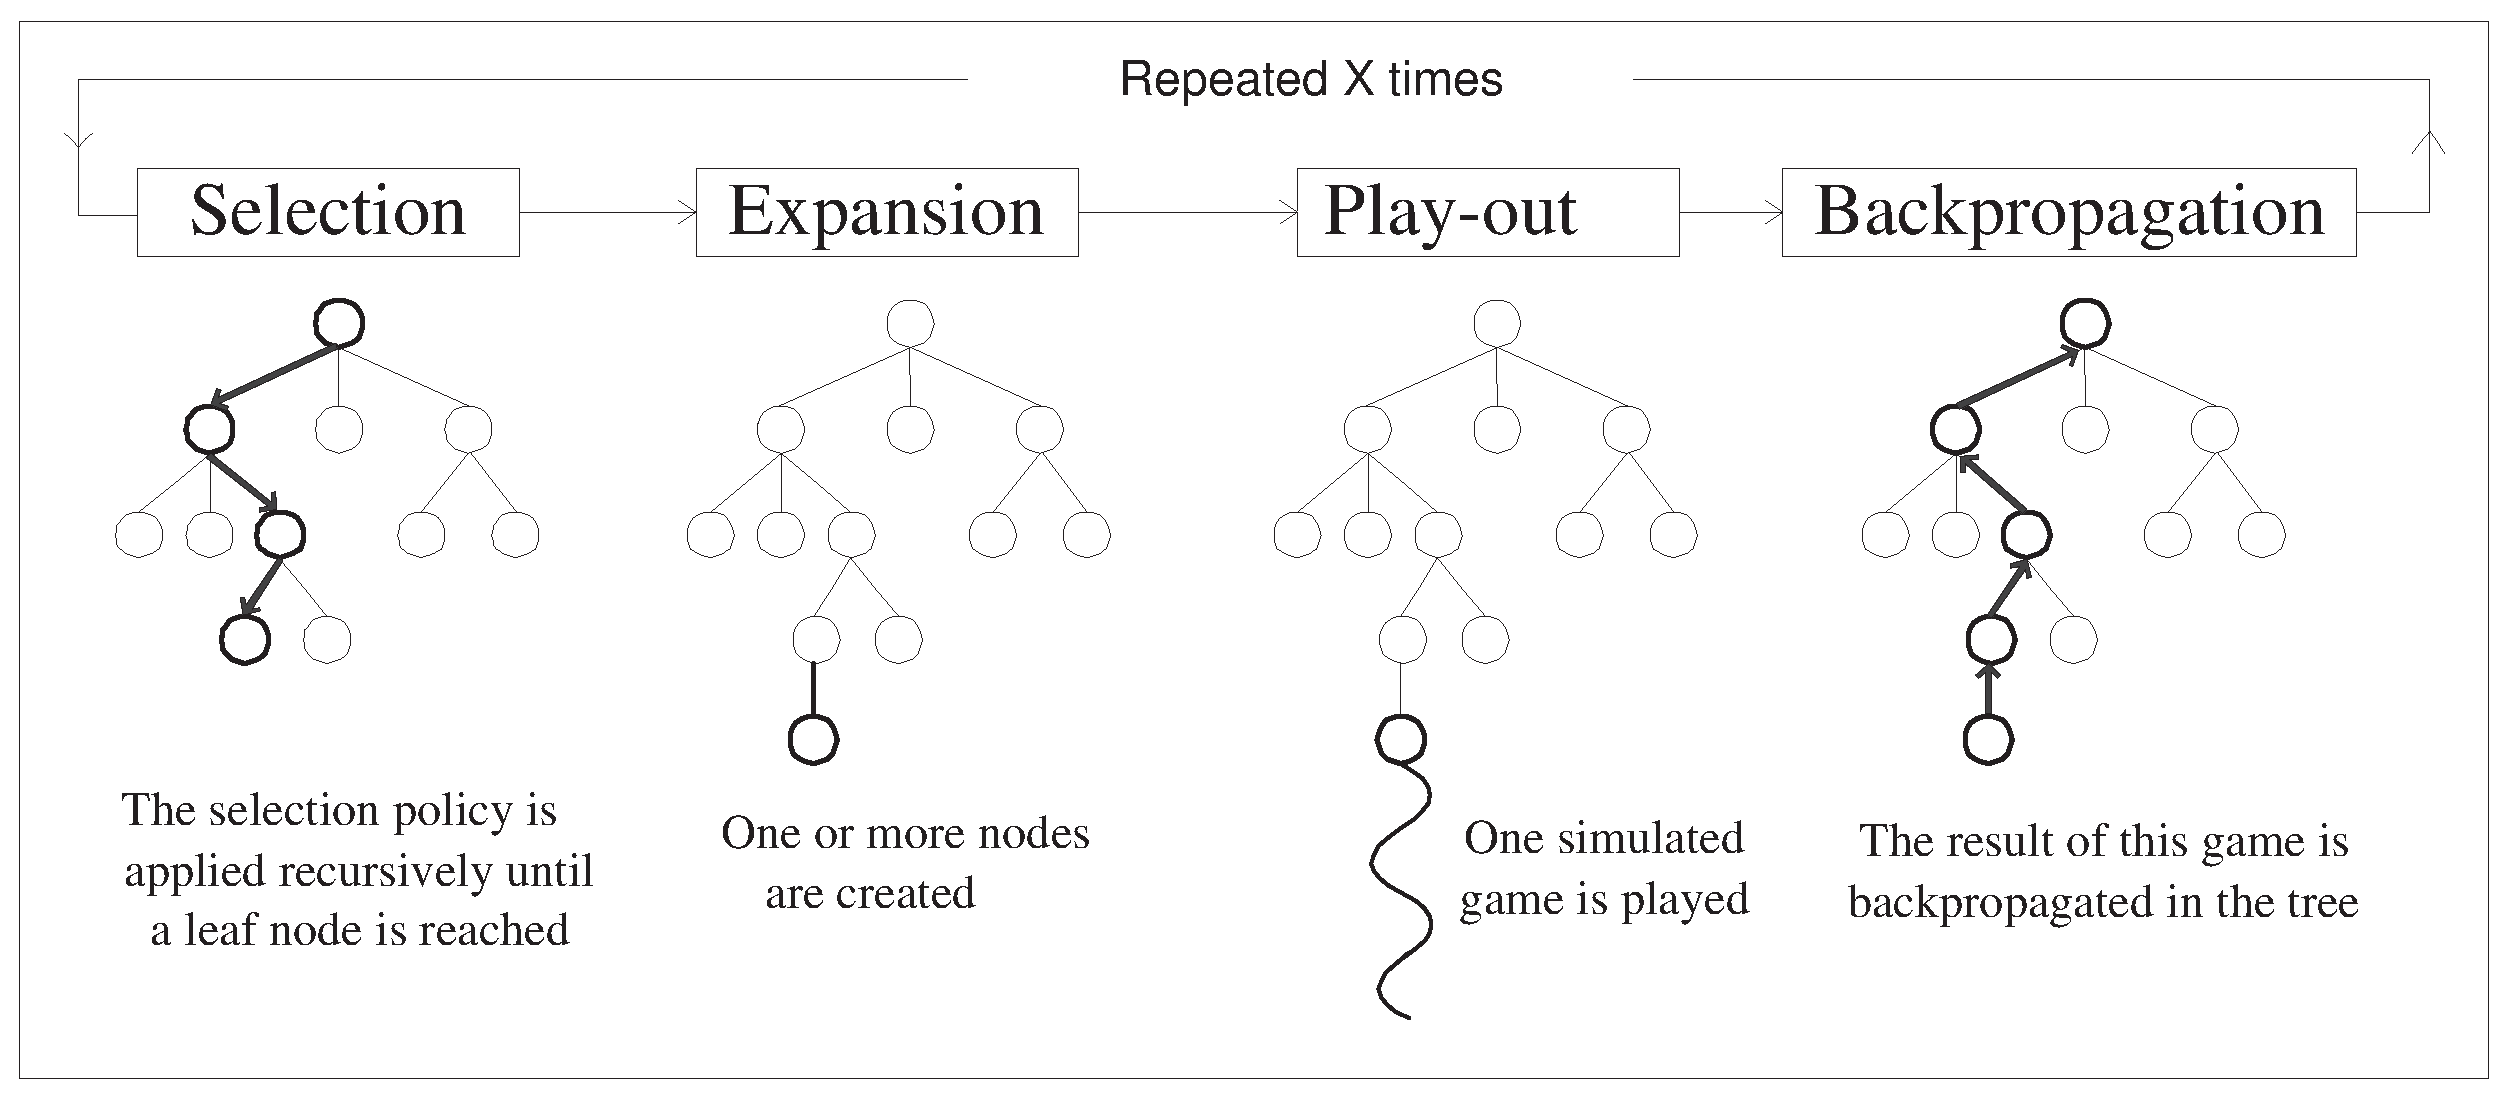
\includegraphics[width=.85\textwidth]{img/figure1.eps}
	\caption{Strategic steps of Monte-Carlo Tree Search~\protect\citebay{chaslot2008progressive}.}
	\label{fig:mcts-algorithm}
\end{figure}

In MCTS, a tree is built incrementally over time which maintains statistics at each node corresponding the rewards collected at those nodes and number of times  they have been visited. The root of this tree corresponds to the current position. The basic version of MCTS consists of four steps, which are performed iteratively until a computational threshold is reached, \ie a set number of iterations, an upper limit on memory usage, or a time constraint. The four steps at each iteration are \citebay{chaslot2008progressive}:
\begin{itemize}
\item {\bf Selection}. Starting at the root node, children are selected recursively according to a selection policy. When a leaf node is reached that does not represent a terminal state it is selected for expansion.
\item {\bf Expansion}. All children are added to the selected leaf node given available moves.
\item {\bf Play-out}. A simulated play-out is run, starting from the state of the added node. Moves are performed randomly or according to a heuristic strategy until a terminal state is reached.
\item {\bf Backpropagation}. The result of the simulated play-out is propagated immediately from the selected node back up to the root node. Statistics are updated along the tree for each node selected during the selection phase and visit counts are increased.
\end{itemize}
The combination of moves selected during the selection step, and the play-out form a single simulation. During the selection step, moves are executed according to the nodes selected in the tree, and during play-out moves are performed randomly, or according to some play-out policy.

Because results are immediately backpropagated, MCTS can be terminated anytime to determine the decision to be made. Moreover, no static heuristic evaluation is required when simulations reach an end state. However, in most cases it is beneficial to add domain knowledge for choosing moves made during the play-out.

The main benefit of MCTS is that it requires no explicit heuristic state evalutation. Rather, states are evaluated by repeatedly sampling them and measuring an average reward. That being said, it is often beneficial to add some domain knowledge to the play-outs such that the simulated games better approximate good play. Moreover, many enhancements to MCTS have been proposed to improve the general performance of the algorithm. Most notably, the MCTS-Solver \citebay{Winands2008} recognises solved wins and losses in the tree and backpropagates their values, RAVE~\citebay{gelly2007} used to speed up node-valuation in the tree, and simulation-policy learning techniques such as low-level $\alpha\beta$ searches~\citebay{Winands2011}, and methods that learn a strategy online, such as the Last-Good-Reply policy~\citebay{baier2010power}, Move-average Sampling Technique (MAST)~\citebay{finnsson2008simulation}, or N-Grams~\citebay{Tak2012}. Combining these techniques often offers greatly improved play by MCTS.

\section{UCT}
\label{uct}
During the selection step, a policy is required to explore the tree to decide on promising options. The Upper Confidence Bound applied to Trees (UCT)~\citebay{kocsis2006bandit} is derived from the UCB1 policy~\citebay{auer2002using} for maximizing the rewards of a multi-armed bandit. In UCT, each node is treated as a bandit problem whose arms are the moves that lead to different child nodes. UCT balances the exploitation of rewarding nodes whilst allowing exploration of lesser visited nodes. Consider a node $p$ with children $I(p)$, then the policy determining which child $i$ to select is defined as:

\begin{equation}
\label{eq:uct}
i^* = argmax_{i \in I(p)}\left\{ v_i + C \sqrt{ \frac{\ln{n_p}}{n_i}}\right\}
\end{equation}
where $v_i$ is the score of the child $i$ based on the average result of simulations that visited it, $n_p$ and $n_i$ are the visit counts of the current node and its child, respectively. $C$ is the exploration constant to tune. 

UCT is applied when the visit count of a child node is above a threshold $T$ generally set to 1. When a node's visit count is below this threshold, a child is selected randomly.

\chapter{Multi-Armed Bandits}
\label{chap:mab}
\begin{chaptercontents} The foundation of simple regret minimization for Monte-Carlo Tree Search (MCTS) is given. Given that MCTS is a recursive multi-armed bandit algorithm, regret minimization in multi-armed bandits is discussed. Moreover the link between simple and cumulative regret is detailed and recent discoveries discussed.
\end{chaptercontents}

\section{Introduction}
The multi-armed bandit (MAB) problem is defined as a stochastic decision making problem \citebay{auer2002using}. An agent is faced with several options, each with their own reward distribution. Based on empirical experimentation a decision to select the option with the best reward distribution. Generally the problem is described as choosing between the most rewarding arm of a multi-armed slot machine found in casino's. The agent can explore by pulling an arm and observing the resulting reward. The reward is drawn from either a fixed or changing propability distribution. Each pull and the returned reward constitutes a trial. 

In the classical MAB setting, the goal is to maximize the cumulative sum of rewards, \ie winning the most money in the slot machine example. Since the agent does not know the distribution of the arms beforehand, he has to \emph{explore} the possible choices, and when a rewarding arm is found, \emph{exploit} this option to gain a high total reward. Generally, after a certain limit, \eg a time-span or number of trials, the agant must return a recommendation to determine the best arm.

The performance of the agent can be evaluated by observing the difference in the rewards obtained over time and the theoretical reward obtained by pulling only the true best arm, called \emph{cumulative regret}. Or, in the case of \emph{simple regret}, observing the difference between the recommended arm and the true best arm, after the forecaster makes its final recommendation.

\section{The Multi-Armed Bandit Problem}
Suppose a trial is setup such that a forecaster (player or agent) has $a \in [[K]] = \{ 1, 2, \cdots , K \}$ actions which can be repeatedly sampled over $t \in [[T]] = \{ 1, 2, \cdots, T \}$ trials. At each step, the forecaster receives a utility $u(a^t) \sim D_a$ according to some underlying distribution $D_a$. Suppose further that the forecaster employs a selection policy $I(t)$ which outputs some $a$ to be sampled at time $t$, and a recommendation policy $J(T)$ which selects the best arm at $T$.

Cumulative regret is defined to be the regret of having not sampled the best single action in hindsight, 
\begin{equation}
R_c^T = \bE \left[ \max_{a' \in [[K]]} \left\{ \sum_{t=1}^T u(a') - \sum_{t=1}^T u(I(t)) \right\} \right].
\end{equation}
In other words, the regret is accumulated at every step of the algorithm.

Now suppose we change the experimental setup and the actions chosen on trials $1, 2, \ldots, T-1$ are taken under some realistic ``simulated environment'' that represents the true online decision problem but without committing to the actions chose, and the only {\it real} decision is made at step $T$ after having played $T-1$ simulations. In contrast, simple regret~\citebay{Bubeck11Pure} quantifies only the regret for the recommentation policy $J$ at time $T$,

\begin{equation}
R_s^T = \bE \left[  \max_{a' \in [[K]]} \left\{ u(a') - u(J(T)) \right\} \right].
\end{equation}

In their analysis of the links between simple and cumulative regret~\citebay{Bubeck11Pure} found that upper bounds on $R_c^T$ lead to lower bounds on $R_s^T$, and that the smaller the upper bound on $R_c^T$, the higher the lower the lower bound on $R_s^T$, regardless of the recommentation policy, \ie the smaller the cumulative regret, the larger the simple regret. As such, no policy can give an optimal guarantee on both simple and cumulative regret at the same time. And in the case of a multi-armed bandit problem the strategy used depends on the context of the problem.

\section{Pure Exploration in Multi-Armed Bandits}

Non-exploiting selection policies have been proposed to decrease simple regret at high rates. Given that UCB has an optimal rate of cumulative regret convergence, and the conflicting limits on the bounds on the regret types shown by~\citebay{Bubeck11Pure}, algorithms that have a higher rate of exploration than UCB will have better bounds on simple regret. 

Consider a uniform selection policy that selects each arm $|K|/T$ times. Assuming that there are $h$ best arms, $(|K|-h)/T$ simulations are spent on inferior arms, and $h/T$ on the best ones. In games for instance, there are often only one or two good moves to be identified, and therefore, when using uniform selection, most time is wasted on pulling sub-optimal arms. Therefore, a more efficient policy is required to ensure that inferior arms are not selected as often as arms with a high utility over time.

Two algorithms have been proposed to solve this problem, and provide both low bounds, and an exponential rate of decrease on simple regret. The first algorithm, Successive Rejects~\citebay{audibert2010best} works by successively removing the single worst arm from the selection. The algorithm computes a budget for each round $n_k$, during the round, each arm is selected an equal number of times. After each round, the empirically worst arm is removed from the selection and a new round started. The lengths of the rounds are computed in such a manner that a specific lower bound on simple regret is guaranteed.\redbold{Should I give the exact rate of error here?} Successive Rejects is detailed in Algorithm \ref{alg:succrej}.

\IncMargin{1em}
\RestyleAlgo{boxruled}
\begin{algorithm2e}[ht]
	\Indm
	\KwIn{total budget $T$, arms $K$}
	\KwOut{recommendation $J_T\in K$}
	\vspace{0.2cm}
	\Indp
	$S_1 \gets \{1,\dots,K\}$, 
	$\widebar{log}(K) \gets \frac{1}{2} + \sum_{i=2}^{K} \frac{1}{i}$
	$n_0 \gets 0$, 																\;
																				\;
	\ForEach{$k\in\{1,\dots,K-1\}$} {
		$n_k = \displaystyle\ceil[\bigg]{\frac{1}{\widebar{log}(K)} \frac{n-K}{K+1-k}}$				\;
	}
																				\;
	\For{k=1 \emph{\KwTo} $|K|-1$}{
		Select each arm $i\in S_k$ $n_k - n_{k-1}$ times 						\;
		$S_{k+1} \gets$ the $|S_k|-1$ empirically best arms from $S_k$			\;
	}
																				\;
	\KwRet{the single element of $S_K$}
  \caption{Successive Rejects~\protect\citebay{audibert2010best}. \label{alg:succrej}}
\end{algorithm2e}
\DecMargin{1em}

A second algorithm, Sequential Halving~\citebay{Karnin13SH} takes a similar approach. As with Successive Rejects, search time is divided into rounds, and during each round arms are pulled equally often. However, instead of removing a single arm from selection after each round, half the arms are removed each time until a single one remains. The rounds in Sequential Halving are equally distributed such that each round has the same number of trials, but with a lower number of available arms. Sequential Halving is detailed in Algorithm \ref{alg:seqhalv}.

\IncMargin{1em}
\RestyleAlgo{boxruled}
\begin{algorithm2e}[ht]
	\Indm
	\KwIn{total budget $T$, arms $K$}
	\KwOut{recommendation $J_T\in K$}
	\vspace{0.2cm}
	\Indp
	$S_0 \gets \{1,\dots,K\}$																\;
	$B \gets \ceil{\log_2{|S|}} - 1$														\;
	\For{k=0 \emph{\KwTo} $B$}{
		sample each arm $i \in S_k$ \newline														
		$n_k = \displaystyle\floor[\bigg]{\frac{T}{|S_k|\ceil{\log_2{|S|}}}}$	\newline					
		times 																				\;
		$S_{k+1} \gets$ the $|S_k|/2$ arms from $S_k$ with the empirically best average		\;
	}
	\KwRet{the single element of $S_B$}
  \caption{Sequential Halving~\protect\citebay{Karnin13SH}. \label{alg:seqhalv}}
\end{algorithm2e}
\DecMargin{1em}

\section{Relation to MCTS}

The widely used selection policy Upper Confidence Bounds (UCB)~\citebay{auer2002using,browne2012survey}, is the foundation of the popular MCTS algorithm, UCT~\citebay{kocsis2006bandit}. The rate of growth of cumulative regret of UCB is $\ln(T)$, which was shown to be optimal rate \citebay{lai1985asymptotically}. Based on this, \citebay{Bubeck11Pure} have shown that a recommendation policy based on such a selection policy suffers a simple regret that decreases at best at a polynomially rate. Hence, if we assume that simple regret is a better measure of the quality of a given decision at time $T$, the general performance of MCTS may be improved by applying a strategy that is focussed on minimizing simple regret fast, rather than cumulative regret.

In the next chapter an algorithm is proposed which uses both simple and cumulative regret minimizing policies at appropriate segments of the MCTS tree. Using this algorithm we can determine whether the assumption that, when using a recursive multi-armed bandit algorithm (MCTS) in games, minimizing simple over cumulative regret is practical and improves overal performance.

\chapter{Simple Reret Based MCTS}
\label{chap:mctssr}
\begin{chaptercontents} The main contribution of this thesis, a novel MCTS algorithm that combines simple and cumulative regret minimizing policies. Issues regarding backpropagation are discussed, and solutions proposed.
\end{chaptercontents}
\section{Introduction}
As a selection policy for MCTS, UCT minimizes cumulative regret over time throughout the tree. At internal nodes, minimizing cumulative regret ensures that  when a rewarding node is identified it is visited more often. Moreover, in the limit UCT converges to a greedy selection policy where at each iteration only the most rewarding node is selected. In effect the average rewards at parent nodes converge to the maximum over their children, \ie UCT converges to maximum backpropagation on a stable distribution \citebay{kocsis2006bandit}. Secondly, UCT ensures that search time is divided efficiently, since pulling suboptimal arms is limited by $\ln(T)$ where $T$ is the number of trials. These two properties are not only practical when long deliberation times are feasable, rather, it is possible to terminate UCT anytime to obtain a reasonable approximation of the utility of a decision. During search this means that at each ply and at any time, MCTS can be asked for a best response to a parent's move.

In contrast, pure exploration algorithms designed to minimize simple regret in multi-armed bandits such as Successive Rejects~\citebay{audibert2010best} and Sequential Halving~\citebay{Karnin13SH}, discussed in Chapter \ref{chap:mab}, explore all options without specifically exploiting the best one. This results in a lower bound on simple regret only after a total of $T$ trials have completed. As such, to be used effectively, these algorithms can not be terminated at any time, and have a lower formal guarantee on the number of suboptimal selections made. Moreover, \citebay{Bubeck11Pure} has shown that at moderate deliberation times, a modified UCB selection policy resulted in better bounds on simple regret. Relating these findings to MCTS, assuming that minimizing simple regret gives an improved rate of error over UCT, we may choose to use a simple regret minimizing algorithm whenever sufficient trials can be performed, and switch to UCT when the computational budget is lower.

Inspired by this analysis, a hybrid algorithm is proposed, named $\mctssr$, which initializes with an explorative depth-limited search, which applies a specific simple regret minimizing policy. Upon reaching its depth limit frontier, where the computational budget per node is lower, the algorithm switches to the UCT selection policy. This algorithm draws from previous work in \citebay{tolpin2012mcts}, where the authors use a simple regret minimizing policy at the root, and UCT throughout the rest of the tree. A recently introduced algorithm SHOT~\citebay{Cazenave14SHOT}, which is an MCTS algorithm based on sequential-halving~\citebay{Karnin13SH} forms the basis for the simple regret part of $\mctssr$. However, where SHOT recursively applies sequential halving throughout the tree, $\mctssr$ uses a simple regret policy (such as sequential halving) only up to a certain depth and UCT elsewhere. 

\redbold{This part needs more on shot and Tolpin and the possible problems with their implementations}

\section{$\mctssr$}

\section{$\mctssr$-SOLVER}

\chapter{Experiments and Results}
\label{chap:experiments}
\begin{chaptercontents}
The $\mctssr$ algorithm is thouroughly evaluated in the following two-player games: Amazons, Breakthrough, Chinese Checkers and Pentalath.
\end{chaptercontents}
\section{Experimental Setup}

\section{Results}

\chapter{Conclusion}
\label{chap:conclusion}

\bibliography{thesis} \emptypage

\appendix

\appchapter{Algorithms}

\appchapter{Detailed results}


\chapterx{Samenvatting} \emptypage

% this can be a translation of the abstract

\end{document}
